\documentclass[a4paper]{article}

\usepackage{pdp}

%------------------------------------------------------------------------------
%	REPORT INFORMATION
%------------------------------------------------------------------------------

\title{ProjectName -- C/Java/Python}
\subtitle{Rapport final}
\author{AIT-ISSAD MOHAMED SAID, BILAL AL FAYOUMI, AMARA KOUSSAY, GUILEM CAUSS}

%------------------------------------------------------------------------------

\begin{document}

%------------------------------------------------------------------------------
%	TITLE PAGE
%------------------------------------------------------------------------------

\maketitle
\thispagestyle{empty}

%------------------------------------------------------------------------------
%	MAIN MATTER
%------------------------------------------------------------------------------

\section*{Introduction}

Lorem ipsum dolor sit amet, consectetur adipiscing elit. Sed do eiusmod tempor
incididunt ut labore et dolore magna aliqua. Ut enim ad minim veniam, quis
nostrud exercitation ullamco laboris nisi ut aliquip ex ea commodo consequat.
Duis aute irure dolor in reprehenderit in voluptate velit esse cillum dolore eu
fugiat nulla pariatur. Excepteur sint occaecat cupidatat non proident, sunt in
culpa qui officia deserunt mollit anim id est laborum.

Pellentesque iaculis molestie euismod. In hac habitasse platea dictumst. Duis eu
gravida sem. Vivamus pulvinar, tellus auctor sollicitudin iaculis, quam massa
blandit ligula, in mollis est tellus et velit. Nulla gravida sapien nibh, nec
faucibus lorem aliquam sed. Curabitur rutrum elit purus, et congue neque
venenatis vitae. Sed non magna nisi. Pellentesque euismod non ipsum a hendrerit.
Pellentesque vehicula tincidunt lacinia. Sed rhoncus porttitor facilisis.

Etiam sed molestie odio. Nunc cursus sollicitudin est vitae posuere. Nullam
pellentesque metus eu dui porttitor bibendum. Morbi egestas arcu ut urna dictum
placerat non non nisl. Quisque non ante in eros cursus pulvinar. Sed augue
libero, eleifend a urna eget, pellentesque condimentum odio. Sed sed dui non
diam mattis interdum eget sed urna. Integer consectetur, erat id rutrum posuere,
dui velit dictum mi, quis tincidunt magna diam sit amet nunc. Etiam dui augue,
sollicitudin rhoncus nisl a, rhoncus tempor purus.

Suspendisse cursus erat et metus fermentum ullamcorper. Etiam eros arcu, dapibus
quis efficitur ut, congue id nunc. Pellentesque aliquam venenatis convallis.
Nulla nisi justo, aliquet quis lacus eget, aliquet maximus velit. Maecenas ex
turpis, iaculis eget dignissim non, efficitur vel mi. Maecenas pharetra elit
ornare sem suscipit ornare id id sapien. Vivamus sem neque, consectetur vitae
aliquet non, finibus eu lectus. Fusce aliquam ipsum ut viverra vehicula. Donec
ultrices varius nulla vel finibus. Donec convallis fringilla ante id porta.

\section{Modélisation du jeu}

\subsection{Représentation de l'état du jeu}

L'état d'une partie est centralisé dans \texttt{GameState}. La classe regroupe
les positions des joueurs, les murs restants et posés, le graphe de
connectivité et le joueur courant. Cette séparation entre état dynamique,
contraintes de déplacement et progression du tour évite de disperser la logique
métier.

Les positions utilisent un encodage linéaire :
\[
\textit{node} = \textit{row} \times \textit{size} + \textit{col}.
\]
Ce format simplifie l'accès aux structures indexées et les parcours. Les champs
utilisés en exécution sont \texttt{board\_size}, \texttt{current\_player},
\texttt{player\_positions}, \texttt{remaining\_walls},
\texttt{vertical\_walls}, \texttt{horizontal\_walls} et \texttt{graph}. Cette
représentation sert directement la validation des coups, l'historisation et la
persistance.

\subsection{Graphe du plateau et structures associées}

Le plateau est modélisé par un graphe non orienté $G=(V,E)$ : les sommets
représentent les cases et les arêtes les déplacements élémentaires autorisés,
conformément à \cite{glendenning2005quoridor,mertens2012quoridor}. Le graphe
est stocké en liste d'adjacence \texttt{dict[int, list[int]]}, adaptée à une
grille creuse (degré maximal $4$) avec un coût mémoire en $O(V+E)$.

Les murs sont appliqués comme suppressions d'arêtes plutôt que comme
transformations géométriques \cite{glendenning2005quoridor}. La vérification de
connectivité repose sur BFS, avec une complexité $O(V+E)$ sur graphe non
pondéré \cite{cormen2009introduction}. Les distances de plus court chemin sont
aussi réutilisées par les heuristiques IA, notamment pour Minimax et MCTS
\cite{ison2018mctsquoridor,mertens2006}.

En complément, le moteur maintient \texttt{player\_positions}, deux collections
de murs (vertical/horizontal) et un historique de snapshots pour
\emph{undo}/\emph{redo}.

\subsection{Déplacements des pions et validation des murs}

Les déplacements de base sont obtenus à partir des voisins du sommet courant
dans le graphe. Lorsqu'un pion adverse occupe un sommet adjacent, la règle de
saut s'applique si la case située derrière reste accessible ; sinon, des
déplacements diagonaux sont autorisés selon les arêtes effectivement présentes.
Ces cas dépendent de l'état courant des pions et sont traités dynamiquement
dans \texttt{pawn\_rules.py}.

La validation d'un mur combine deux contrôles : validité locale de placement
(position, orientation, absence de chevauchement) et maintien d'un chemin vers
la zone cible pour chaque joueur. L'implémentation effectue une suppression
temporaire des arêtes concernées, exécute un BFS par joueur, puis valide la
pose ou restaure l'état précédent. Sur une grille $9\times 9$, ce coût reste
faible.

Le modèle retenu établit un lien direct entre structures de données et règles
d'exécution : le graphe représente la connectivité, les règles dynamiques
gèrent les cas contextuels et les vérifications globales assurent la validité
de la partie.

\section{Architecture logicielle}

\subsection{Architecture générale}

Les Figures~\ref{fig:uml-main} et~\ref{fig:uml-io-ai} présentent les composants
principaux du projet en deux vues lisibles.

\begin{figure}[htbp]
  \centering
  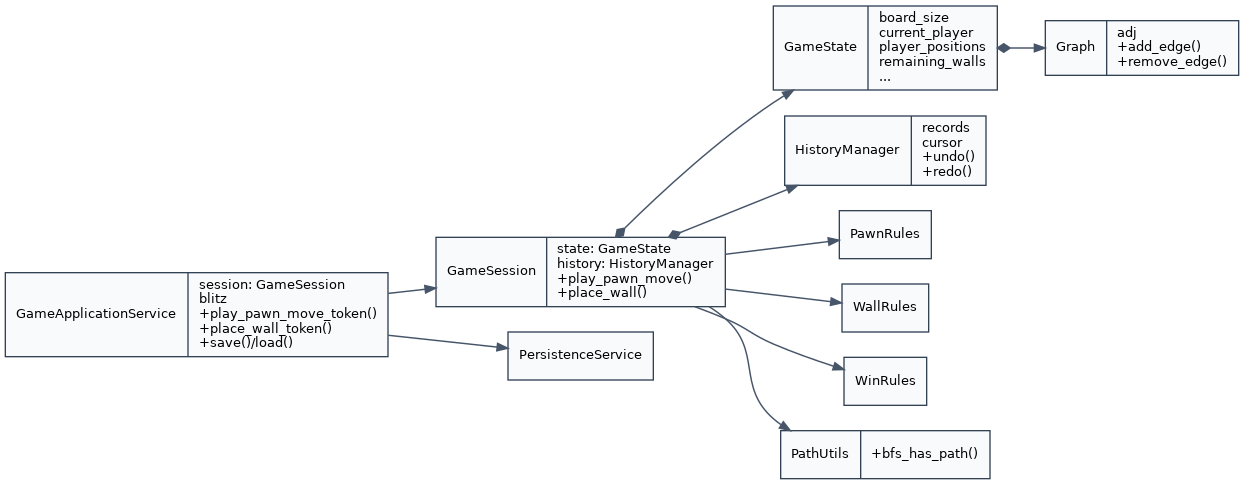
\includegraphics[width=\textwidth]{quoridor_uml_main.png}
  \caption{Vue UML du noyau métier et de la couche applicative}
  \label{fig:uml-main}
\end{figure}

\begin{figure}[htbp]
  \centering
  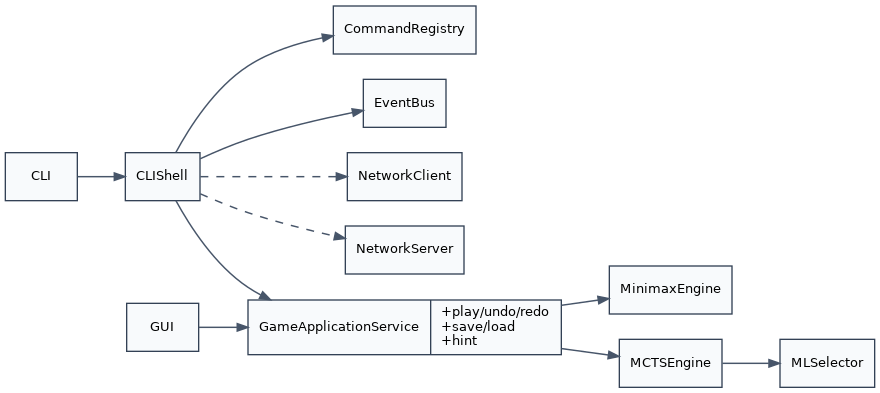
\includegraphics[width=\textwidth]{quoridor_uml_io_ai.png}
  \caption{Vue UML des interfaces, du réseau et des composants IA}
  \label{fig:uml-io-ai}
\end{figure}

L'architecture est organisée en couches : les modules d'interface et de réseau
passent par la couche applicative, qui orchestre les opérations métier.
\texttt{GameState} porte l'état, \texttt{GameSession} applique les transitions
et \texttt{GameApplicationService} constitue le point d'entrée commun pour CLI,
GUI, IA, persistance et réseau.

\subsection{Modules et dépendances}

Le module \texttt{core} contient le modèle métier (état, plateau, notation,
snapshots). Le module \texttt{rules} implémente les validations de
déplacements, de murs et de victoire. Le module \texttt{application} orchestre
les cas d'usage et le cycle de partie. Les modules \texttt{interfaces} et
\texttt{network} gèrent l'entrée/sortie utilisateur et les échanges
client/serveur. Le module \texttt{utils} regroupe les composants techniques
réutilisables (graphe, utilitaires), et \texttt{ml} porte les composants d'aide
aux moteurs de recherche.

Les dépendances restent dirigées : \texttt{interfaces} $\rightarrow$
\texttt{application} $\rightarrow$ (\texttt{core}, \texttt{rules},
\texttt{utils}), avec \texttt{network} connecté à \texttt{application}. Cette
orientation limite les cycles et isole le coeur métier.

\begin{verbatim}
quoridor/
|-- core/
|-- rules/
|-- application/
|-- interfaces/
|-- network/
`-- ml/
\end{verbatim}

\subsection{Cheminement des actions}

Toutes les actions passent par le même pipeline applicatif. Pour un déplacement
utilisateur : interface $\rightarrow$ \texttt{GameApplicationService}
$\rightarrow$ validation \texttt{rules} $\rightarrow$ mise à jour
\texttt{GameSession}/\texttt{GameState} $\rightarrow$ historisation via
\texttt{HistoryManager} $\rightarrow$ retour interface.

La pose de mur suit la même chaîne, avec simulation sur graphe et test BFS
avant validation. Un coup IA suit également ce pipeline :
\texttt{GameApplicationService} déclenche Minimax/MCTS, puis applique le coup
sélectionné via les mêmes étapes de validation et de mise à jour.

\subsection{Intégration des algorithmes}

BFS est implémenté dans \texttt{rules}/\texttt{utils} pour les tests de
connectivité. Les moteurs Minimax, alpha-bêta et MCTS sont orchestrés par
\texttt{application}. Le mécanisme \emph{undo}/\emph{redo} repose sur
\texttt{HistoryManager} et les snapshots d'état. La persistance et le parsing
assurent la conversion entre formats externes et représentation interne, sans
dupliquer la logique métier.

\subsection{Design patterns utilisés}

\paragraph{Command}
Dans le shell CLI, les commandes et \texttt{CommandRegistry} encapsulent les
actions utilisateur et délèguent leur exécution à
\texttt{GameApplicationService}. Cette structure découple saisie et exécution.

\paragraph{Strategy}
\texttt{PlayCommandStrategy}, \texttt{LocalPlayCommandStrategy} et
\texttt{NetworkPlayCommandStrategy} isolent les variantes d'exécution
local/réseau, sans multiplier les conditions dans la couche applicative.

\paragraph{Memento}
\texttt{GameSnapshot}, \texttt{MoveRecord} et \texttt{HistoryManager}
conservent les états avant/après action, ce qui permet des restaurations
cohérentes pour \emph{undo}/\emph{redo}.

\paragraph{Facade}
\texttt{GameApplicationService} joue le rôle de façade : il expose une API
unique pour jouer un coup, poser un mur, gérer l'historique, piloter l'IA et
charger/sauvegarder une partie.

\paragraph{Observer}
\texttt{EventBus} implémente un mécanisme d'observation léger entre producteurs
et consommateurs d'événements, utile pour propager les mises à jour sans
dépendances directes fortes.

L'ensemble produit une architecture compacte : responsabilités localisées,
dépendances orientées vers le métier, et extensions (IA, réseau, interfaces)
ajoutées sans modifier le noyau de règles.

\section*{Conclusion}

Suspendisse sit amet nisi placerat, vestibulum nisl vel, iaculis nunc.
Suspendisse quis libero vel ipsum gravida congue nec id arcu. Donec vel mi
viverra, commodo urna vitae, tincidunt lectus. Fusce pellentesque, lectus a
placerat vestibulum, magna lectus placerat nibh, vehicula pellentesque lacus
erat non nulla. Suspendisse maximus, turpis at suscipit egestas, libero massa
ultrices libero, at tincidunt velit eros a eros. Maecenas id tempor nunc.
Phasellus condimentum porttitor sapien in sagittis. Proin in metus diam. Mauris
in turpis sed ex viverra iaculis. Sed lobortis, tellus vitae congue blandit, leo
elit auctor libero, id tempor ante dolor quis quam. Donec eget ligula quam.
Maecenas porttitor massa vel felis elementum tristique.

%------------------------------------------------------------------------------
%	BIBLIOGRAPHY
%------------------------------------------------------------------------------

\nocite{*}
\bibliographystyle{plain}
\bibliography{bibliography}

%------------------------------------------------------------------------------
% BACK MATTER
%------------------------------------------------------------------------------
\appendix

\section{Section en annexe}

Lorem ipsum dolor sit amet, consectetur adipiscing elit. Sed do eiusmod tempor
incididunt ut labore et dolore magna aliqua. Ut enim ad minim veniam, quis
nostrud exercitation ullamco laboris nisi ut aliquip ex ea commodo consequat.
Duis aute irure dolor in reprehenderit in voluptate velit esse cillum dolore eu
fugiat nulla pariatur. Excepteur sint occaecat cupidatat non proident, sunt in
culpa qui officia deserunt mollit anim id est laborum.

\end{document}
